\documentclass{ximera}
%% You can put user macros here
%% However, you cannot make new environments

\listfiles

\graphicspath{{./}{firstExample/}{secondExample/}}

\usepackage{tikz}
\usepackage{tkz-euclide}
\usepackage{tikz-3dplot}
\usepackage{tikz-cd}
\usetikzlibrary{shapes.geometric}
\usetikzlibrary{arrows}
\usetkzobj{all}
\pgfplotsset{compat=1.13} % prevents compile error.

%\renewcommand{\vec}[1]{\mathbf{#1}}
\renewcommand{\vec}{\mathbf}
\newcommand{\RR}{\mathbb{R}}
\newcommand{\dfn}{\textit}
\newcommand{\dotp}{\cdot}
\newcommand{\id}{\text{id}}
\newcommand\norm[1]{\left\lVert#1\right\rVert}
 
\newtheorem{general}{Generalization}
\newtheorem{initprob}{Exploration Problem}

\tikzstyle geometryDiagrams=[ultra thick,color=blue!50!black]

%\DefineVerbatimEnvironment{octave}{Verbatim}{numbers=left,frame=lines,label=Octave,labelposition=topline}



\usepackage{mathtools}


\title{Where was Eye? (part 3)} \license{CC BY-NC-SA 4.0}

\begin{document}

\begin{abstract}
We determine the location of the camera based on a photograph it took.
\end{abstract}
\maketitle

\section*{Where was Eye? (part 3)}


We will now develope a theoretical foundation for our method of figuring out the height of the camera. 

\begin{exploration}\label{exp:hideAndSeek}
Suppose Alice, Bob, Colin, Daria, and Evan are playing hide-and-seek in the school yard.  Alice is the seeker.  The diagram below shows the location of the players.  Which of the children is visible to Alice?
     \begin{image}
         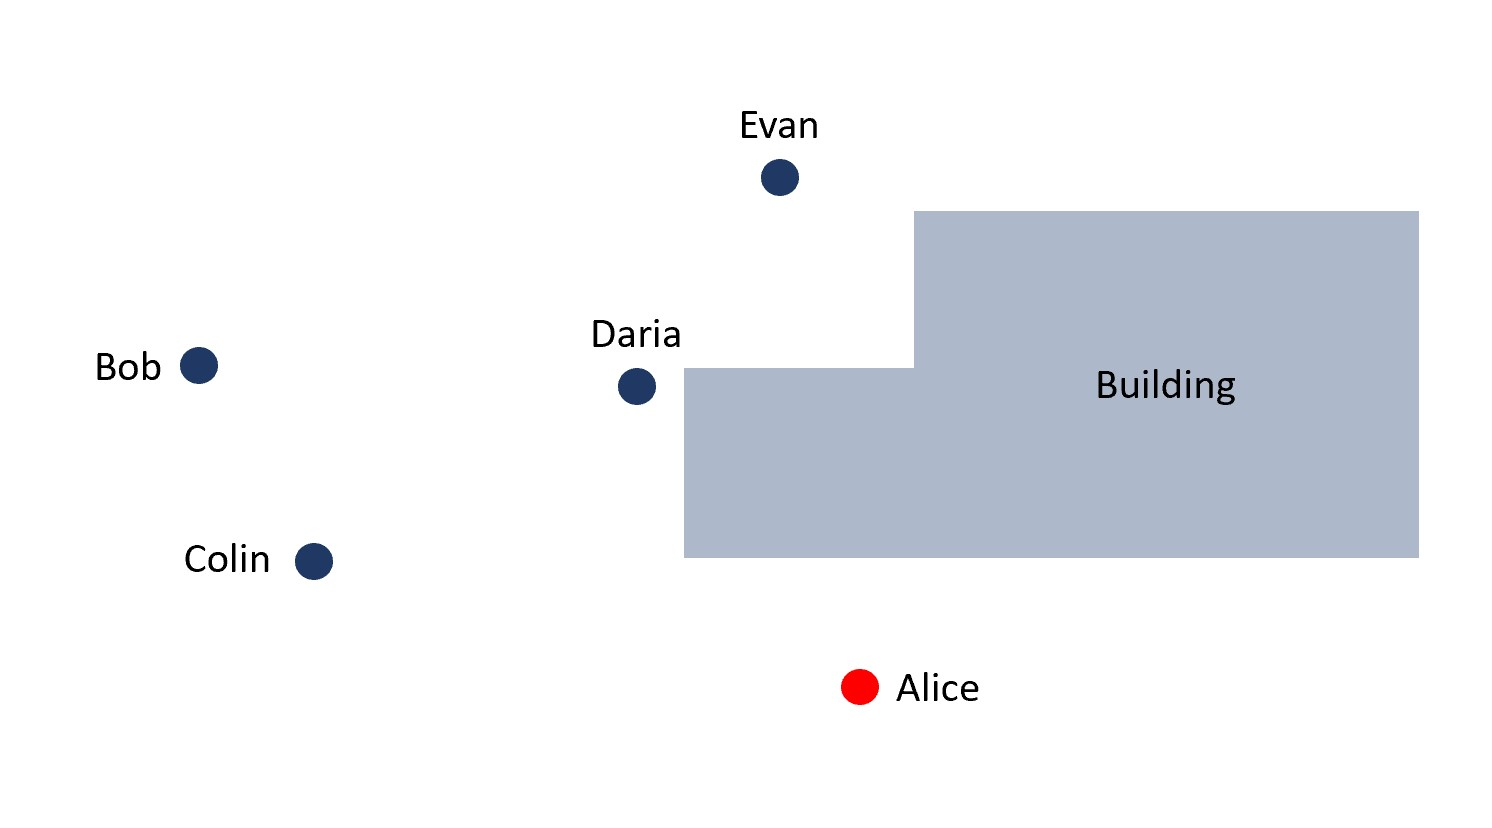
\includegraphics[width=5in]{hideAndSeek1.jpg}
\end{image}
Check the name of all children that Alice can see.
\begin{selectAll}
\choice[correct]{Bob}
\choice[correct]{Colin}
\choice{Daria}
\choice{Evan}
\end{selectAll}

\textbf{Group Discussion Prompt:}
\emph{Articulate the reason for your choices.  If you need help formulating your thoughts, click on the arrow (below, right), and use the diagram to help you.}

\begin{expandable}
    \begin{image}
         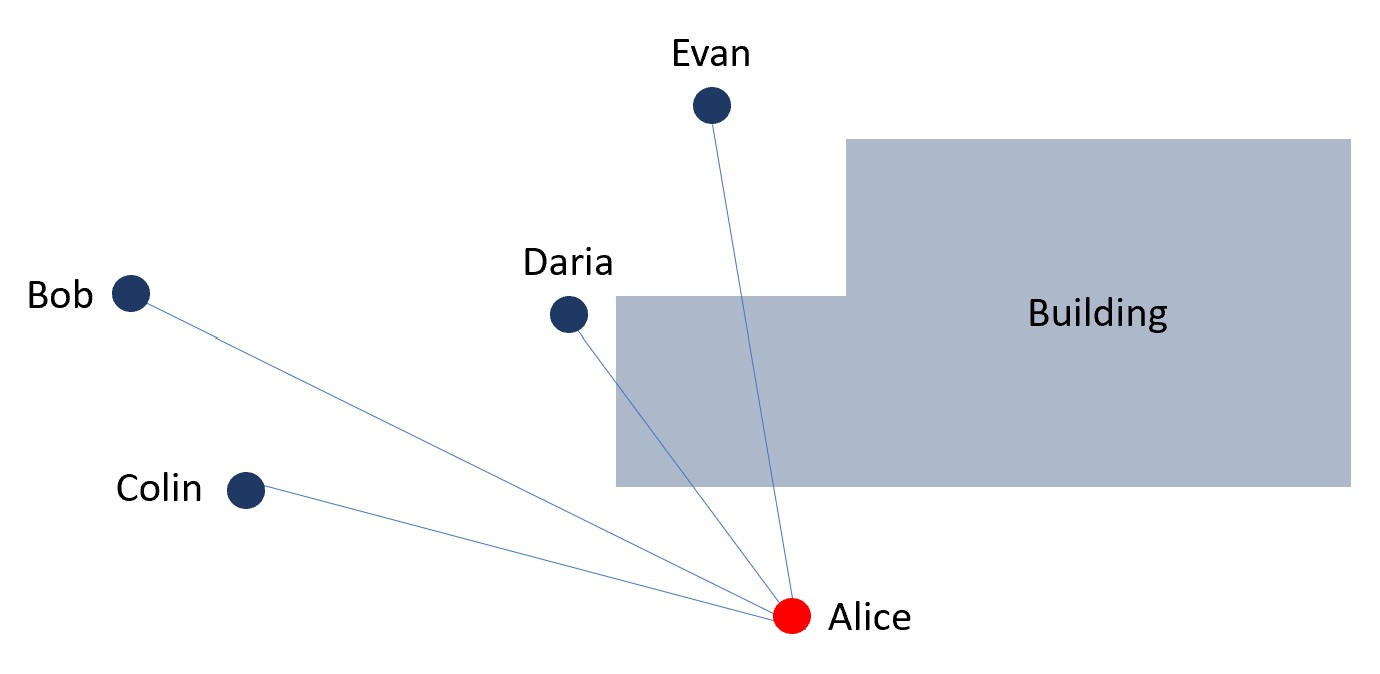
\includegraphics[width=5in]{hideAndSeek2.jpg}
\end{image}
\end{expandable}
\end{exploration}

The above exploration intuitively established a very important fact: we see along straight lines.  These lines are called \emph{lines of sight}.
\begin{image}
         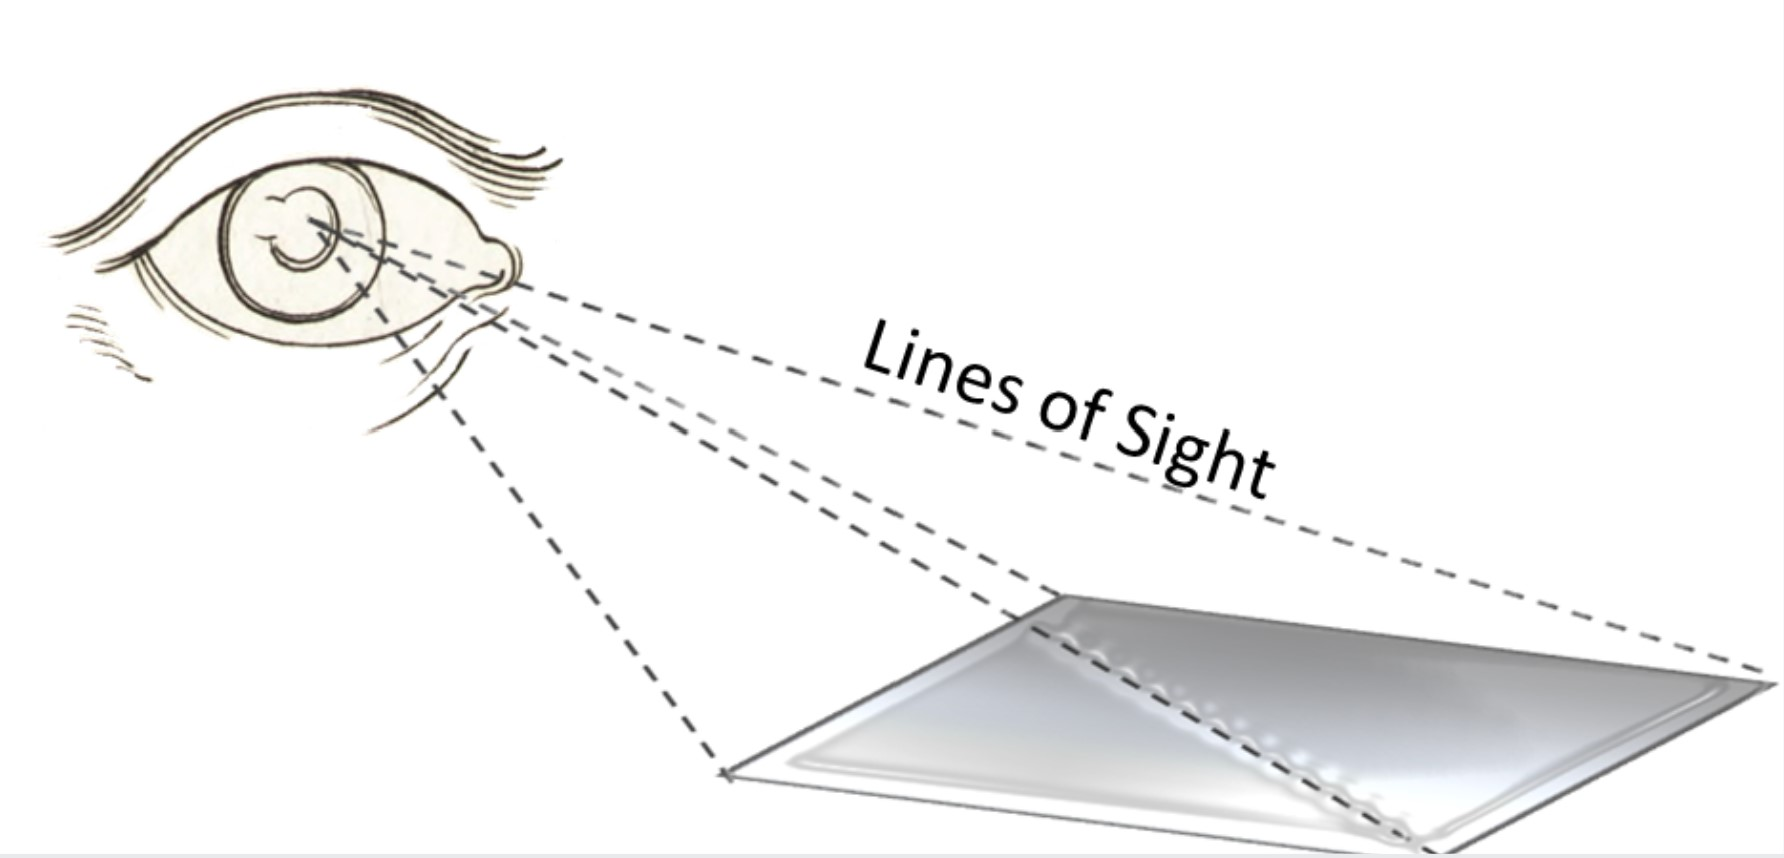
\includegraphics[width=5in]{linesOfSight.jpg}
\end{image}


\end{document}